\section{Desarrollo experimental}

Para el desarrollo de la práctica se armó un circuito RLC en serie con la finalidad de observar experimentalmente el fenómeno de resonancia eléctrica. El circuito estuvo formado por una resistencia, una bobina y un capacitor conectados en serie. La señal de alimentación fue proporcionada mediante un generador de funciones, configurado para entregar una señal senoidal. La respuesta del circuito se observó con un osciloscopio digital, utilizando dos canales: uno para medir la señal de entrada y otro para medir la señal de salida sobre la resistencia.

La medición de la salida en la resistencia se realizó debido a que, en un circuito serie, la corriente es la misma en todos los elementos. Por lo tanto, el voltaje en la resistencia es directamente proporcional a la corriente del circuito, de acuerdo con la ley de Ohm:

\[
V_R = RI
\]

De esta forma, al observar el voltaje en la resistencia fue posible analizar el comportamiento de la corriente al variar la frecuencia de excitación.

\begin{figure}[H]
	\centering
	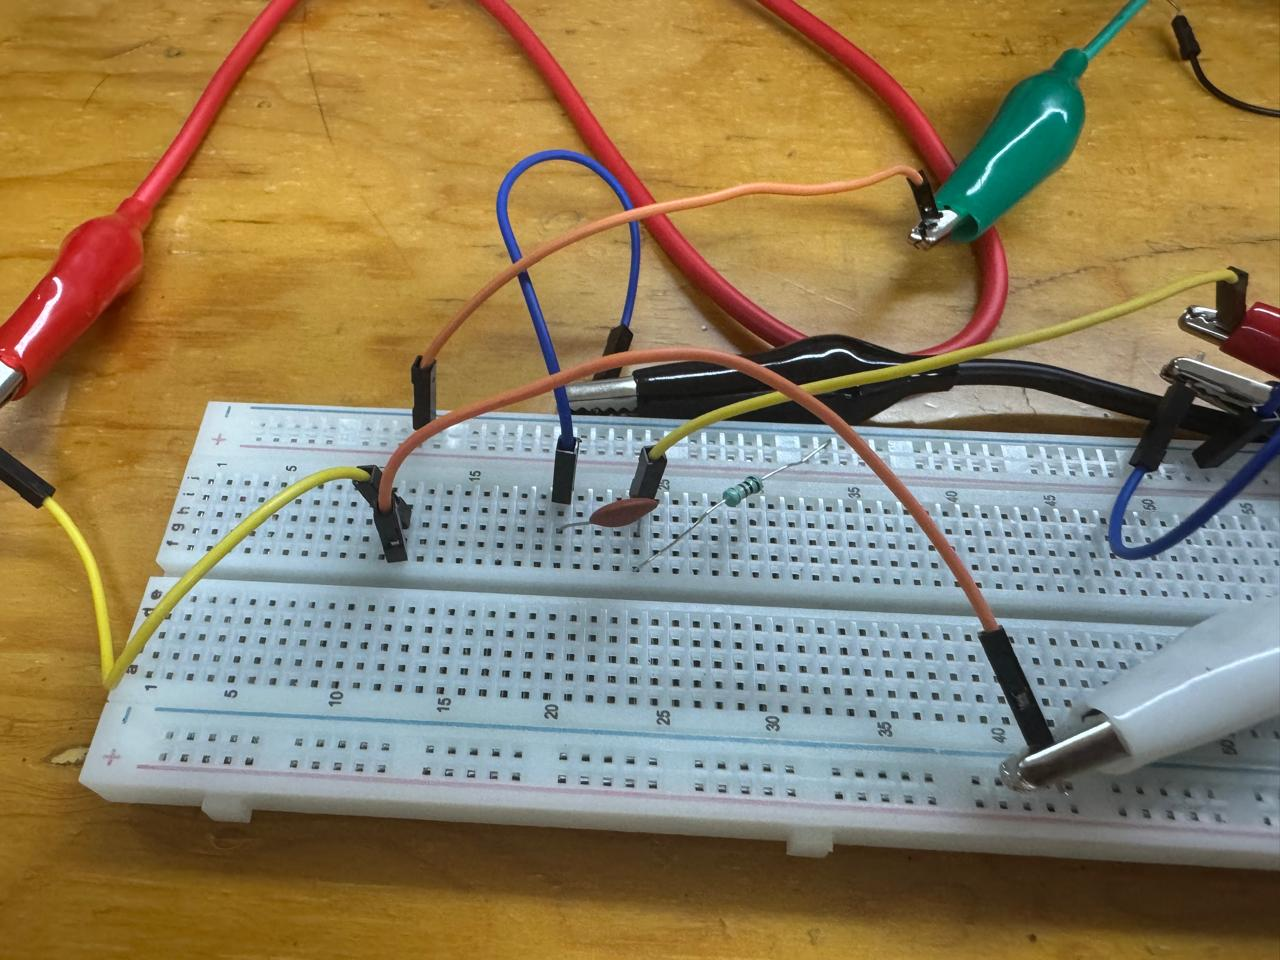
\includegraphics[width=0.75\linewidth]{assets/img/montaje_rlc.jpg}
	\caption{Montaje físico del circuito RLC en serie en protoboard.}
	\label{fig:montaje_rlc}
\end{figure}

Los valores utilizados para el circuito fueron:

\[
R = 1~k\Omega
\]

\[
C = 0.22~\mu F
\]

\[
L = 32.4~mH
\]

Además, se consideró la resistencia interna de la bobina, la cual fue aproximadamente:

\[
R_L = 32.4~\Omega
\]

Por lo tanto, la resistencia total efectiva del circuito se puede expresar como:

\[
R_T = R + R_L
\]

\[
R_T = 1000~\Omega + 32.4~\Omega = 1032.4~\Omega
\]

\begin{table}[H]
	\centering
	\begin{tabular}{|c|c|}
		\hline
		\textbf{Elemento} & \textbf{Valor} \\ \hline
		Resistencia & $1~k\Omega$ \\ \hline
		Capacitor & $0.22~\mu F$ \\ \hline
		Inductor & $32.4~mH$ \\ \hline
		Resistencia interna de la bobina & $32.4~\Omega$ \\ \hline
	\end{tabular}
	\caption{Valores de los componentes utilizados en la práctica.}
	\label{tab:componentes}
\end{table}

Una vez armado el circuito, se conectó el generador de funciones a la entrada del arreglo RLC. La amplitud de la señal de entrada se mantuvo aproximadamente constante durante las mediciones, con un valor cercano a:

\[
V_{i,pp} \approx 5~V
\]

Posteriormente, se conectaron las puntas del osciloscopio para observar simultáneamente la señal de entrada y la señal de salida. En las mediciones se utilizó una escala vertical de $2~V/div$ para ambos canales, lo cual permitió comparar visualmente la amplitud y el desfase entre las dos señales.

El procedimiento consistió en variar gradualmente la frecuencia de la señal senoidal hasta localizar tres puntos importantes del comportamiento del circuito: la frecuencia inferior de corte, la frecuencia de resonancia y la frecuencia superior de corte.

\subsection{Determinación de la frecuencia de resonancia}

La frecuencia de resonancia se identificó observando el punto en el que las señales de entrada y salida se encontraron prácticamente en fase. En esta condición, la reactancia inductiva y la reactancia capacitiva se compensan entre sí:

\[
X_L = X_C
\]

\[
\omega L = \frac{1}{\omega C}
\]

Por lo tanto, la parte imaginaria de la impedancia total se anula y el circuito se comporta como una carga principalmente resistiva:

\[
Z = R_T
\]

En el osciloscopio se observó que, al ajustar la frecuencia cerca de $1.54~kHz$, el desfase entre los canales fue prácticamente cero. En esta condición, el voltaje de salida sobre la resistencia alcanzó uno de sus valores más altos, lo cual indica que la corriente del circuito fue máxima.

\[
f_0 \approx 1.54~kHz
\]

\[
\theta \approx 0^\circ
\]

\begin{figure}[H]
	\centering
	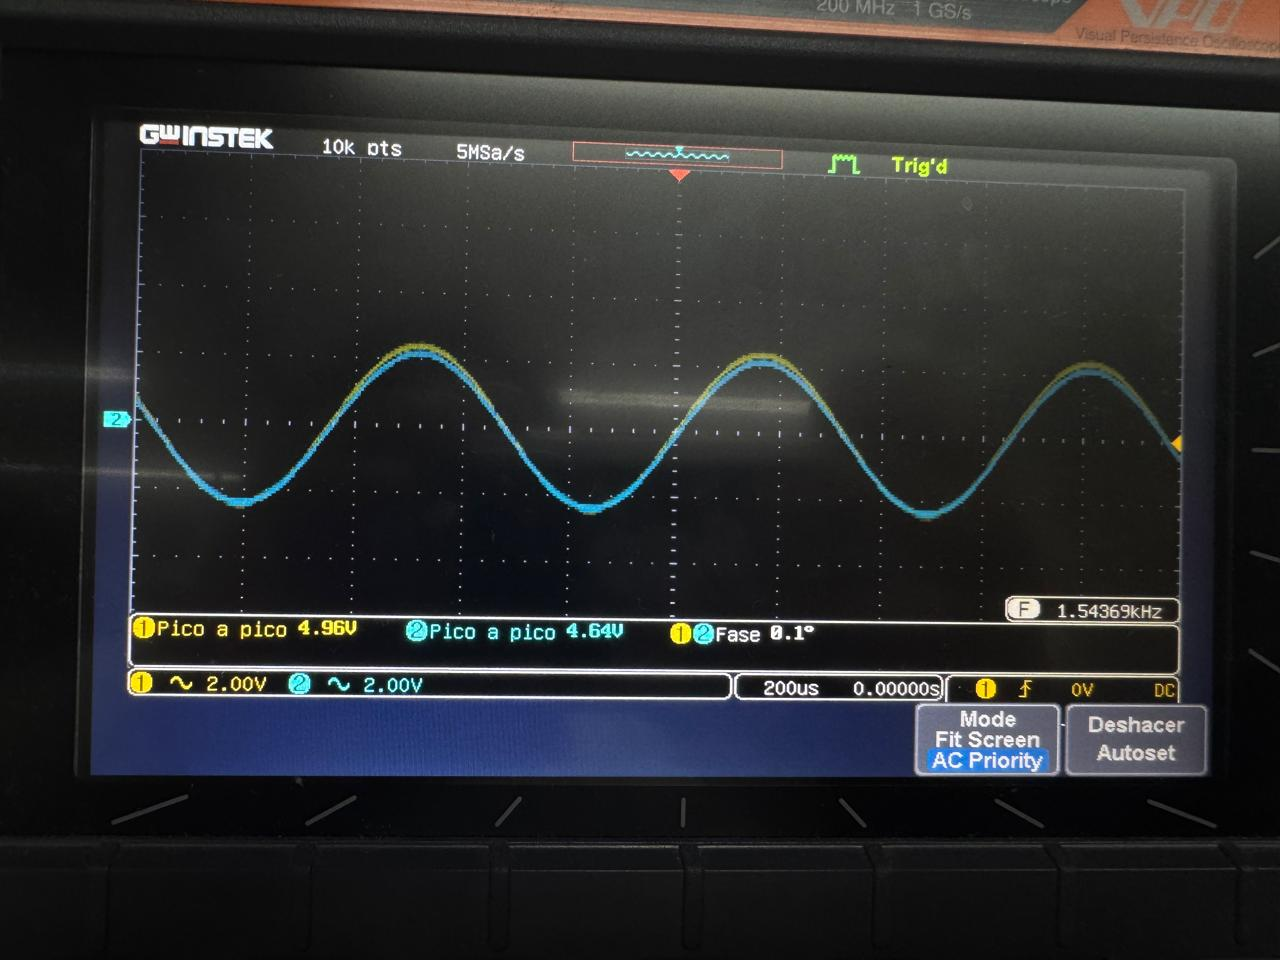
\includegraphics[width=0.78\linewidth]{assets/img/resonancia_154khz.jpg}
	\caption{Señales de entrada y salida aproximadamente en fase durante la resonancia.}
	\label{fig:resonancia}
\end{figure}

En la imagen anterior se aprecia que ambas señales tienen prácticamente la misma posición horizontal, por lo que el desfase es cercano a cero. Esto confirma que el circuito se encuentra en resonancia. Para esta condición se registraron los siguientes valores aproximados:

\[
f_0 = 1.543~kHz
\]

\[
V_{i,pp} \approx 4.96~V
\]

\[
V_{o,pp} \approx 4.64~V
\]

La frecuencia angular correspondiente se calculó mediante:

\[
\omega_0 = 2\pi f_0
\]

\[
\omega_0 = 2\pi(1543)
\]

\[
\omega_0 \approx 9695~rad/s
\]

\subsection{Frecuencia inferior de corte}

Después de localizar la frecuencia de resonancia, se disminuyó gradualmente la frecuencia del generador hasta encontrar el punto en el cual el desfase entre la señal de entrada y la señal de salida fue aproximadamente de $-45^\circ$. Este punto corresponde a la frecuencia inferior de corte del circuito.

Experimentalmente se observó que esta condición ocurrió aproximadamente en:

\[
f_1 \approx 563.7~Hz
\]

\[
\theta \approx -45^\circ
\]

\begin{figure}[H]
	\centering
	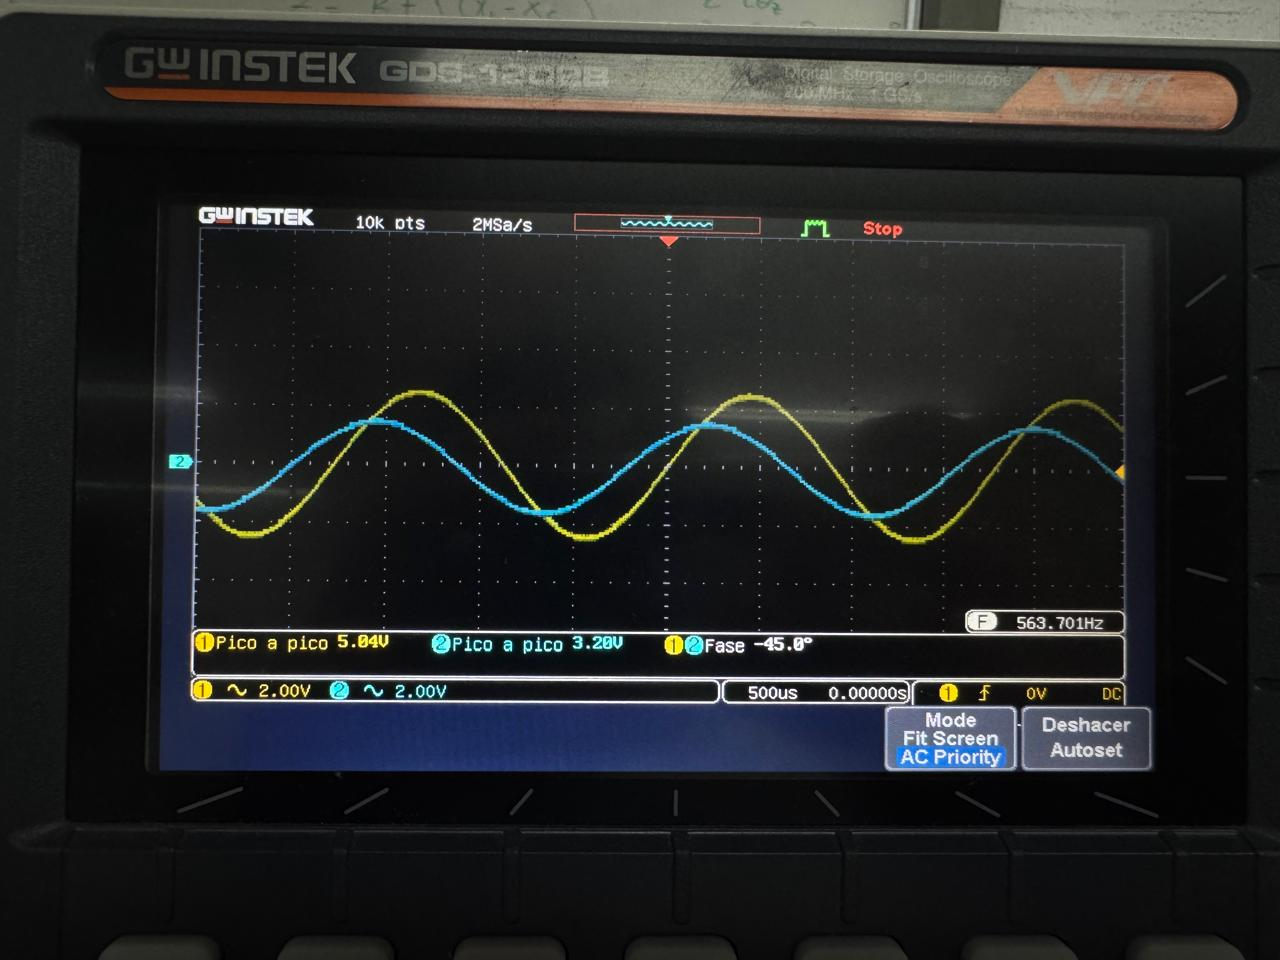
\includegraphics[width=0.78\linewidth]{assets/img/corte_inferior_563Hz.jpg}
	\caption{Medición de la frecuencia inferior de corte con desfase aproximado de $-45^\circ$.}
	\label{fig:corte_inferior}
\end{figure}

En esta región de baja frecuencia, el circuito presenta un comportamiento predominantemente capacitivo, ya que la reactancia capacitiva es mayor que la reactancia inductiva. Por esta razón, la corriente se adelanta respecto al voltaje de entrada y aparece un desfase negativo en la medición.

Para esta frecuencia se registraron aproximadamente los siguientes valores:

\[
f_1 = 563.7~Hz
\]

\[
V_{i,pp} \approx 5.04~V
\]

\[
V_{o,pp} \approx 3.20~V
\]

La frecuencia angular correspondiente fue:

\[
\omega_1 = 2\pi f_1
\]

\[
\omega_1 = 2\pi(563.7)
\]

\[
\omega_1 \approx 3541~rad/s
\]

\subsection{Frecuencia superior de corte}

Posteriormente, se aumentó la frecuencia del generador, pasando nuevamente por la frecuencia de resonancia, hasta encontrar el punto donde el desfase entre las señales fue aproximadamente de $45^\circ$. Este punto corresponde a la frecuencia superior de corte.

De acuerdo con la medición observada en el osciloscopio, la frecuencia superior de corte fue aproximadamente:

\[
f_2 \approx 3.713~kHz
\]

\[
\theta \approx 45^\circ
\]

\begin{figure}[H]
	\centering
	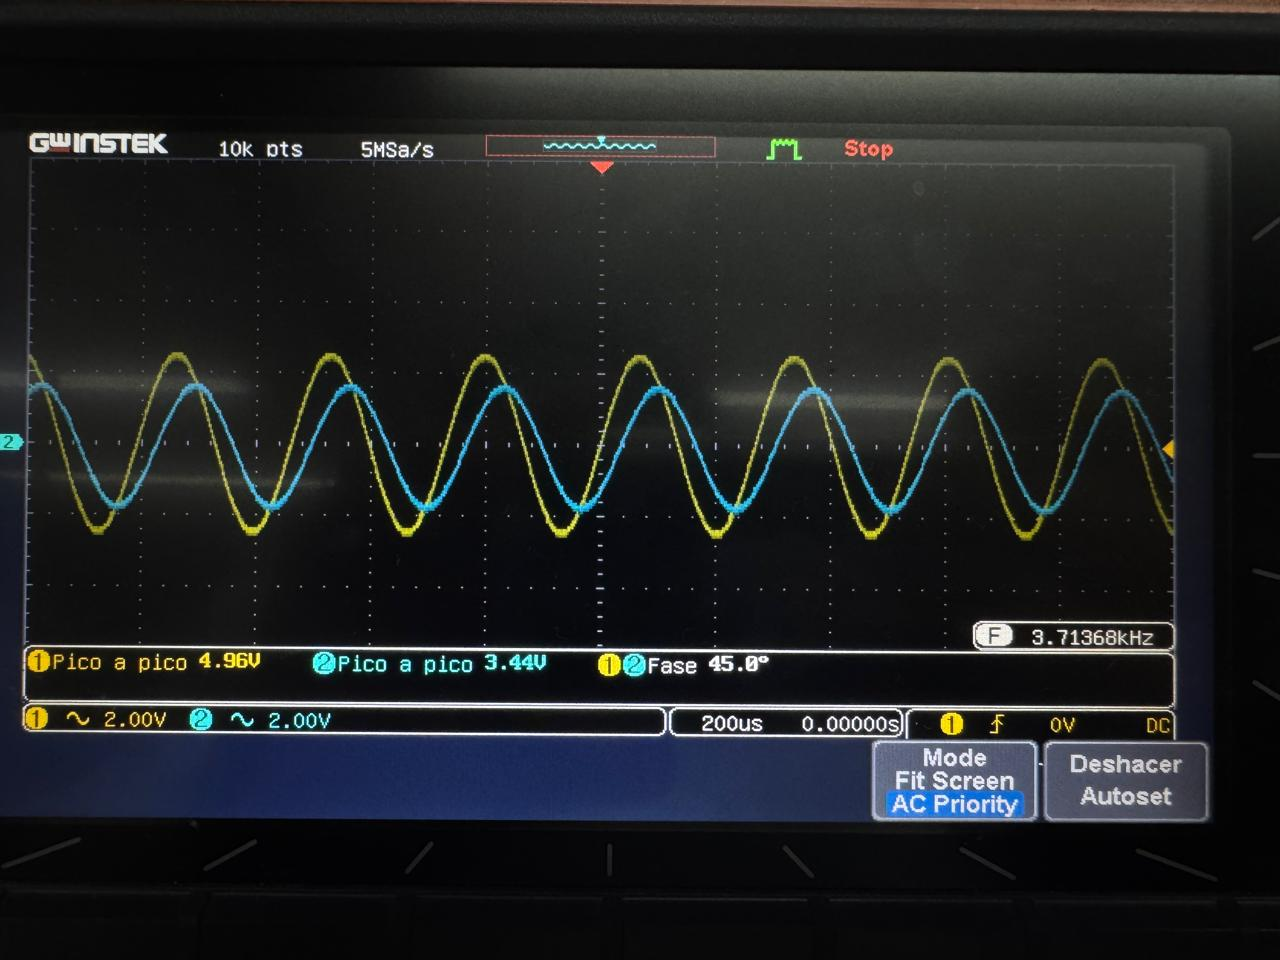
\includegraphics[width=0.78\linewidth]{assets/img/corte_superior_3713Hz.jpg}
	\caption{Medición de la frecuencia superior de corte con desfase aproximado de $45^\circ$.}
	\label{fig:corte_superior}
\end{figure}

En esta región de alta frecuencia, el circuito presenta un comportamiento predominantemente inductivo, debido a que la reactancia inductiva aumenta con la frecuencia. Como consecuencia, la corriente se retrasa respecto al voltaje de entrada y el desfase observado es positivo.

Los valores aproximados registrados fueron:

\[
f_2 = 3713.7~Hz
\]

\[
V_{i,pp} \approx 4.96~V
\]

\[
V_{o,pp} \approx 3.44~V
\]

La frecuencia angular correspondiente fue:

\[
\omega_2 = 2\pi f_2
\]

\[
\omega_2 = 2\pi(3713.7)
\]

\[
\omega_2 \approx 23335~rad/s
\]

\subsection{Ancho de banda y factor de calidad}

Con las frecuencias de corte obtenidas experimentalmente, se calculó el ancho de banda del circuito:

\[
AB = f_2 - f_1
\]

\[
AB = 3713.7 - 563.7
\]

\[
AB \approx 3150~Hz
\]

El factor de calidad experimental se obtuvo mediante:

\[
Q = \frac{f_0}{AB}
\]

\[
Q = \frac{1543}{3150}
\]

\[
Q \approx 0.49
\]

Este valor indica que el circuito presenta una respuesta de baja selectividad, ya que el ancho de banda es relativamente grande en comparación con la frecuencia de resonancia. Esto significa que el circuito no responde únicamente en una frecuencia muy estrecha, sino que permite una respuesta considerable en un intervalo amplio de frecuencias.

\subsection{Tabla de datos experimentales}

A partir de las mediciones realizadas con el osciloscopio, se resumen los principales valores obtenidos:

\begin{table}[H]
	\centering
	\begin{tabular}{|c|c|c|c|c|}
		\hline
		\textbf{Condición} & \textbf{Frecuencia} & \textbf{Desfase} & \textbf{$V_{i,pp}$} & \textbf{$V_{o,pp}$} \\ \hline
		Frecuencia inferior de corte & $563.7~Hz$ & $-45^\circ$ & $5.04~V$ & $3.20~V$ \\ \hline
		Resonancia & $1.543~kHz$ & $0^\circ$ & $4.96~V$ & $4.64~V$ \\ \hline
		Frecuencia superior de corte & $3.713~kHz$ & $45^\circ$ & $4.96~V$ & $3.44~V$ \\ \hline
	\end{tabular}
	\caption{Datos experimentales obtenidos durante la práctica.}
	\label{tab:datos_experimentales}
\end{table}

\subsection{Análisis del comportamiento observado}

Los resultados obtenidos muestran el comportamiento esperado para un circuito RLC serie. A bajas frecuencias, el capacitor domina el comportamiento del circuito, por lo que se observa un desfase negativo entre la señal de entrada y la señal de salida. Al aumentar la frecuencia, la reactancia inductiva también aumenta, mientras que la reactancia capacitiva disminuye. Cuando ambas reactancias se igualan en magnitud, la parte reactiva de la impedancia se anula y el circuito entra en resonancia.

En la frecuencia de resonancia, las señales de entrada y salida se observaron prácticamente en fase, lo cual indica que la impedancia del circuito fue principalmente resistiva. Además, el voltaje medido en la resistencia fue máximo, confirmando que la corriente también alcanzó su valor más alto.

Después de la resonancia, al seguir aumentando la frecuencia, el comportamiento del circuito se volvió inductivo. Esto se manifestó mediante un desfase positivo cercano a $45^\circ$ en la frecuencia superior de corte.

Finalmente, el valor obtenido para el factor de calidad confirma que el circuito no fue altamente selectivo. Esta condición puede atribuirse a la resistencia del circuito, a la resistencia interna de la bobina, a las tolerancias de los componentes y a pérdidas parásitas presentes en el montaje físico.